%!TEX root = ../thesis.tex

\begin{table*}
  \centering
  % \tiny
  % \fontfamily{phv}
  % \begin{tabular}{*{2}{|c}|r*{13}{|c}|}
  %   \hline
  %   \multicolumn{1}{|p{0.008\columnwidth}|}{\centering{ID}} &
  %   \multicolumn{1}{|p{0.03\columnwidth}|}{\centering{Editing expertise (years)}} &
  %   \multicolumn{1}{|p{0.04\columnwidth}|}{\centering{Footage length}} &
  %   \multicolumn{1}{|p{0.04\columnwidth}|}{\centering{Demo-Cut video length}} &
  %   \multicolumn{1}{|p{0.04\columnwidth}|}{\centering{Final video length}} &
  %   \multicolumn{1}{|p{0.04\columnwidth}|}{\centering{Anno-tation time (mins)}} &
  %   \multicolumn{6}{|p{0.35\columnwidth}|}{\centering{\# and types of markers used for annotation}} &
  %   \multicolumn{1}{|p{0.03\columnwidth}|}{\centering{Ave text length (words)}} &
  %   \multicolumn{1}{|p{0.03\columnwidth}|}{\centering{\# of segments}} &
  %   \multicolumn{1}{|p{0.04\columnwidth}|}{\centering{Review \& edit time (mins)}} &
  %   \multicolumn{1}{|p{0.03\columnwidth}|}{\centering{\# of effects changed}} \\
  %   \cline{7-12} & & & & & & Total & Step & Action & Supply & Closeup & Cutout & & & & \\ \hline
  %   P1 & 5 & 3'51" & 2'14" & 2'14" & 10 & 20 & 3 & 10 & 5 & 1 & 1 & 3.2 & 28 & 8 & 1 \\
  %   P2 & 3 & 7'16" & 4'09" & 4'14" & 16 & 29 & 4 & 16 & 4 & 5 & 0 & 4 & 49 & 11 & 4 \\
  %   P3 & 10 & 10'57" & 6'45" & 6'45" & 18 & 36 & 10 & 18 & 4 & 0 & 4 & 2.2 & 57 & 10 & 3 \\
  %   P4 & 2 & 9'16" & 5'12" & 5'38" & 25 & 35 & 6 & 20 & 3 & 4 & 2 & 3.3 & 56 & 13 & 6 \\ \hline
  %   P5 & 0 & 7'17" & 4'13" & 4'07" & 17 & 38 & 5 & 18 & 7 & 6 & 2 & 3 & 56 & 12 & 5\\
  %   P6 & 0 & 6'28" & 3'20" & 2'48" & 8 & 24 & 3 & 13 & 6 & 0 & 2 & 3.5 & 40 & 9 & 9 \\
  %   P7 & 0 & 10'08" & 6'18" & 6'02" & 21 & 66 & 7 & 35 & 12 & 8 & 4 & 3.9 & 92 & 14 & 20 \\
  %   P8 & 0 & 8'58" & 3'05" & 3'03" & 8 & 13 & 4 & 6 & 1 & 0 & 2 & 3.6 & 21 & 10 & 2 \\ \hline
  %   AVE & 2.5 & 8'01" & 4'24" & 4'21" & 15 & 33 & 5 & 17 & 5 & 3 & 2 & 3.3 & 50 & 11 & 6 \\ \hline
  % \end{tabular}

  \centering
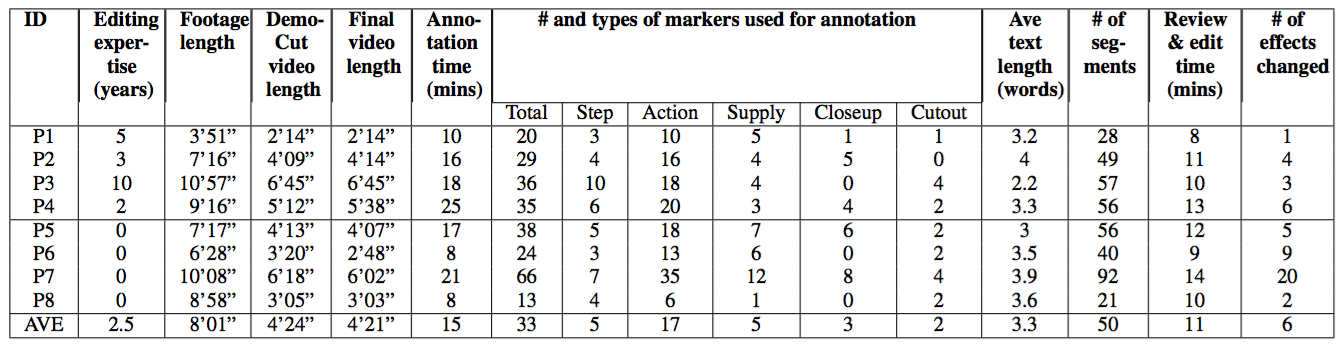
\includegraphics[width=\columnwidth]{\democut/fig/study_evaluation}
  \caption{Quantitative analysis of the user evaluation.}
  \label{tab:table2}
\end{table*}

% https://docs.google.com/spreadsheet/ccc?key=0Ak-N9HjmbtiYdHdNc01aZ3RoWllmN1puQ2VrOXhmNFE&usp=sharing

\subsection{Discussion}
All of the participants successfully created a complete video tutorial
of their gift wrapping technique using DemoCut during the study
session. The average length of the recorded demonstrations was 8
minutes, and the final generated videos were just over 5 minutes long
(45\% shorter than the raw footage). On average, participants spent 15
minutes annotating the recordings and added 33
markers. Table~\ref{tab:table2} summarizes several other quantitative
results from the study.

Here, we summarize a few key points from the responses to the
questionnaire and the end-of-study discussions:

\subsubsection{DemoCut interface and workflow.}
We received strong positive
feedback about the DemoCut interface as a whole and the editing
workflow that it enables. All participants agreed or strongly agreed that
it was easy to annotate a recording using the Annotation Interface, and seven
of them found it easy to use the reviewing and Editing Interface.
%
P1 explained, \iquote{This is very simple for beginning users and
  takes out some of the guess work around learning how to use
  different layers, speed effects, etc.},
and P2 described the workflow as, \iquote{super easy and SUPER FAST!}
%
P6 also appreciated the simplicity of the interface: \iquote{I like
  this a lot because there aren't thousands of different buttons to
  work with.}
%
In addition, several participants noted how the automated components
of the system reduced the amount of effort required to create an
edited video: \iquote{I could be lazier and still have a great video
  cause it did everything for me} (P8), and \iquote{Pre-segmentation
  (when it worked well) made it easy to zero in on the portion I
  wanted to modify} (P4).

\subsubsection{Automatic editing effects.} In general, the participants
liked how DemoCut automatically removed or condensed parts of their
recordings. Their feedback suggests that the automatically generated
effects were particularly useful for speeding up repetitive actions
like cutting and folding and skipping extraneous actions, such as removing
the adhesive sticker from a bow. As P3 noted, these effects were generally successful because
DemoCut \iquote{correctly understood parts with no speech but long
  actions.} Another participant commented specifically
on the fast motion with merged audio effect, and said \iquote{(I)
  appreciate the automatic speeding up/slowing down of video to match
  speech.} %\wl{which one?} \pc{pilot user...}

\subsubsection{Reviewing and editing.} As expected, there were some cases where
participants decided to modify the automatic effects. Errors in the audio analysis can cause the narration within a
segment to get cut off when fast motion effects are applied.  To eliminate these
audio artifacts, participants changed the segment effect from fast
motion to normal mode. In cases where the narration referred to
specific visual events, participants switched from the default fast
motion with merged audio effect to leap frog with synchronized
audio. Finally, in a few situations, participants decided to skip an
annotated segment that they deemed unnecessary or unclear after
reviewing the rest of the tutorial.

\subsubsection{Quality of generated tutorials.} Five of the eight
participants said they were satisfied or very satisfied with the video
tutorials that they created with DemoCut during the study.
%\wl{Peggy/Joyce: it would be nice to say the following things, but I'm not sure if they are true. Please take a look and edit as necessary.}
%\md{assuming peggy and choice looked at this and edited given that 3 hours until the deadline.}
The remaining three participants had significantly more video
editing experience, and they wanted to further refine their tutorials
by adjusting some of the timing and cut points using more traditional
low-level editing tools.
%
However, even these participants agreed that DemoCut was
\iquote{good for a first pass of editing} and provided \iquote{helpful
  ``smart'' suggestions} even though the system is \iquote{limited in
  manual control.}

\subsubsection{Default speed-up effects.} The participants noted some limitations
with the default editing effects. P5 explained that \iquote{having the speed up of video be
  the default speed creates a stressful tutorial.} Some
participants pointed out that there are some obvious cases where fast
motion with merged audio should not be applied; for example, the
effect \iquote{does not work well if the person's face is showing
  (the speech and mouth movements would not match up).} We agree with
these comments and plan to use face detection and add an adaptive learner to
improve the system. % \md{not sure what you mean by ``pause'' markers? We don't have markers in the editing phase.}
%\md{who said this?}  pilot
% \md{I don't understand this. When would you add a pause marker - in the editing interface?}

\subsubsection{Annotation guidelines.} One observation from the study is that
adding too many markers during the annotation phase can hurt the
quality of the generated tutorial. Adding markers temporally close together leads to many short
segments, and since DemoCut applies a video edit effect to each segment
individually, the resulting tutorial may end up transitioning rapidly
through several inconsistent effects (e.g., fast motion effects with
various playback speeds). One way to address this problem is to make
automatic editing decisions that span several consecutive segments. The
participants offered a few other suggestions: P4 wonders \iquote{if
  there are simple tips you could give to the user while recording
  that would make them more successful,} and P8 suggested that seeing
real-time effects while adding markers might help him
understand how best to annotate the recording.

% quotes: https://docs.google.com/document/d/15kd3invJgX5JK1I3wkLBJf3eHSGL37C1IbSeUkXiIvE/edit?usp=sharing
% P1-P4:
% * How satisfied were you with the suggested automatic video edits our system performed after you added annotations? 3.25
% * Were you satisfied with the video effects? 3.75
% * Were you satisfied with the audio concentration if there was any? How easy was it to edit the tutorial using this interface? 3
% * Were you satisfied with your final video output? 3.75
% * Would you post this on YouTube under your own YouTube username? 2 Yes / 2 No
% * In general, how easy was it to use this system to create video instructional tutorials? 3.75
